Un autódromo tiene la forma y las dimensiones que ilustra la figura \ref{fig:autodromo}.
\begin{figure}[H]
    \centering
    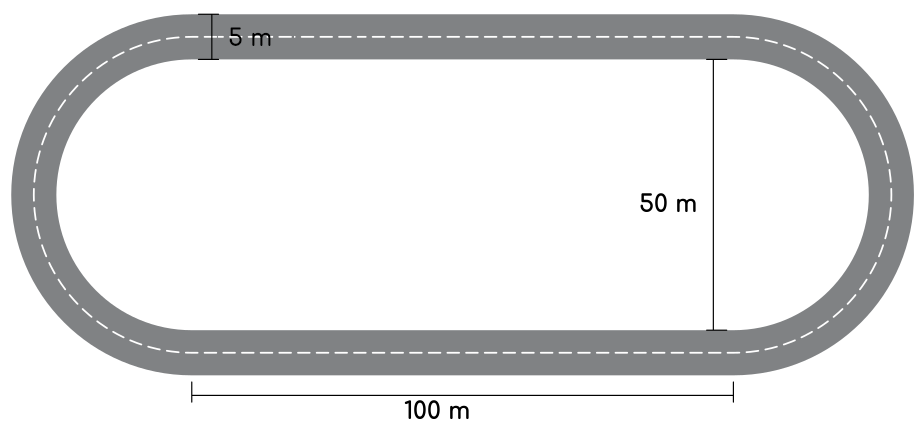
\includegraphics[width=.8\linewidth]{../images/autodromo}
    \captionof{figure}{Diagrama de la pista de carreras en el autódromo.}
    \label{fig:autodromo}
\end{figure}
\begin{parts}
    \part Calcula la distancia que cubre un auto al recorrer una vez el circuito por el carril interno.

    \begin{solutionbox}{3cm}

    \end{solutionbox}

    \part Calcula la distancia que se recorre en un auto al conducir una vez por el carril externo.

    \begin{solutionbox}{3cm}

    \end{solutionbox}

    \part A qué distancia se deben separar dos autos en una carrera de una vuelta para que ambos recorran la misma distancia.

    \begin{solutionbox}{3cm}

    \end{solutionbox}
\end{parts}